% --------------------------------------------------------------
% This is all preamble stuff that you don't have to worry about.
% Head down to where it says "Start here"
% --------------------------------------------------------------
 
\documentclass[12pt]{article}

\usepackage[margin=1in]{geometry} 
\usepackage{amsmath,amsthm,amssymb}
\usepackage{float}
\usepackage{graphicx}
\usepackage[bookmarks]{hyperref}
\usepackage{listings}
\usepackage{color}
\usepackage{enumitem}
\usepackage{tikz}
\usetikzlibrary{calc,arrows.meta,positioning}

\tikzset{
	every node/.style={font=\sffamily\small},
	main node/.style={thick,circle,draw,font=\sffamily\Large}
}

\definecolor{codegreen}{rgb}{0,0.6,0}
\definecolor{codegray}{rgb}{0.5,0.5,0.5}
\definecolor{codepurple}{rgb}{0.58,0,0.82}
\definecolor{backcolour}{rgb}{0.95,0.95,0.92}

\lstdefinestyle{mystyle}{
	backgroundcolor=\color{backcolour},   
	commentstyle=\color{codegreen},
	keywordstyle=\color{magenta},
	numberstyle=\tiny\color{codegray},
	stringstyle=\color{codepurple},
	basicstyle=\footnotesize,
	breakatwhitespace=false,         
	breaklines=true,                 
	captionpos=b,                    
	keepspaces=true,                 
	numbers=left,                    
	numbersep=5pt,                  
	showspaces=false,                
	showstringspaces=false,
	showtabs=false,                  
	tabsize=2
}

\lstset{style=mystyle}

\newcommand{\N}{\mathbb{N}}
\newcommand{\Z}{\mathbb{Z}}
\newcommand{\R}{\mathbb{R}}

\newenvironment{theorem}[2][Theorem]{\begin{trivlist}
		\item[\hskip \labelsep {\bfseries #1}\hskip \labelsep {\bfseries #2.}]}{\end{trivlist}}
\newenvironment{lemma}[2][Lemma]{\begin{trivlist}
		\item[\hskip \labelsep {\bfseries #1}\hskip \labelsep {\bfseries #2.}]}{\end{trivlist}}
\newenvironment{exercise}[2][Exercise]{\begin{trivlist}
		\item[\hskip \labelsep {\bfseries #1}\hskip \labelsep {\bfseries #2.}]}{\end{trivlist}}
\newenvironment{reflection}[2][Reflection]{\begin{trivlist}
		\item[\hskip \labelsep {\bfseries #1}\hskip \labelsep {\bfseries #2.}]}{\end{trivlist}}
\newenvironment{proposition}[2][Proposition]{\begin{trivlist}
		\item[\hskip \labelsep {\bfseries #1}\hskip \labelsep {\bfseries #2.}]}{\end{trivlist}}
\newenvironment{corollary}[2][Corollary]{\begin{trivlist}
		\item[\hskip \labelsep {\bfseries #1}\hskip \labelsep {\bfseries #2.}]}{\end{trivlist}}
 
\begin{document}
 
% --------------------------------------------------------------
%                         Start here
% --------------------------------------------------------------
 
%\renewcommand{\qedsymbol}{\filledbox}
 
\title{Making the Markov Random Field}%replace X with the appropriate number
\author{Abhi Devathi} %if necessary, replace with your course title
 
\maketitle
 
% --------------------------------------------------------------
%     You don't have to mess with anything below this line.
% --------------------------------------------------------------
 
\begin{center}
	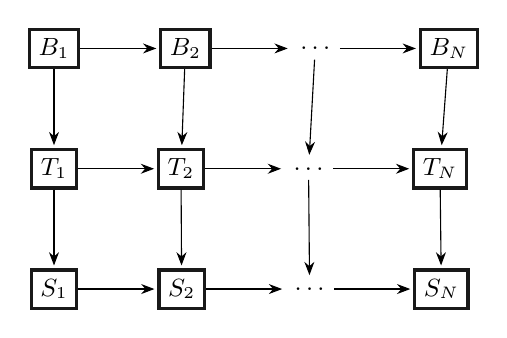
\begin{tikzpicture}[->, >={Stealth[sep]}, distance=2.9cm,
	squarednode/.style={rectangle, draw=black!90, very thick},]
	\node[squarednode] (1) {$B_1$};
	\node[squarednode] (2) [right =of 1]{$B_2$};
	\node[] (3) [right =of 2]{$\ldots$};
	\node[squarednode] (4) [right =of 3]{$B_N$};

	\node[squarednode] (5) [below =of 1]{$T_1$};
	\node[squarednode] (6) [right =of 5]{$T_2$};
	\node[] (7) [right =of 6]{$\ldots$};
	\node[squarednode] (8) [right =of 7]{$T_N$};
	
	\node[squarednode] (9) [below =of 5]{$S_1$};
	\node[squarednode] (10) [right =of 9]{$S_2$};
	\node[] (11) [right =of 10]{$\ldots$};
	\node[squarednode] (12) [right =of 11]{$S_N$};
	
	% Horizontal Arrows
	\draw (1) -- (2);
	\draw (2) -- (3);
	\draw (3) -- (4);
	
	\draw (5) -- (6);
	\draw (6) -- (7);
	\draw (7) -- (8);
	
	\draw (9)  -- (10);
	\draw (10) -- (11);
	\draw (11) -- (12);
	
	% Vertical Arrows
	\draw (1) -- (5);
	\draw (5) -- (9);
	
	\draw (2) -- (6);
	\draw (6) -- (10);	
	
	\draw (3) -- (7);
	\draw (7) -- (11);
	
	\draw (4) -- (8);
	\draw (8) -- (12);
	\end{tikzpicture}
\end{center}

\end{document}
